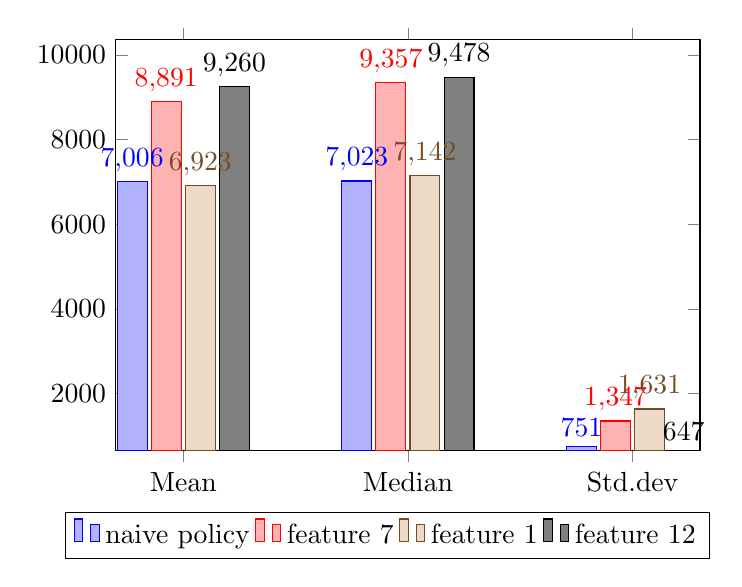
\begin{tikzpicture}

\begin{axis}[
    ybar = 1.5pt,
    enlargelimits=0.15,
    height = 6.8cm, width = 9cm,
    bar width = 0.38cm,
    enlarge y limits={value=.1,upper},
    legend style={at={(0.465,-0.15)},
    anchor=north,legend columns=-1},
    symbolic x coords={Mean,Median,Std.dev},
    y tick label style={/pgf/number format/.cd,%
          scaled y ticks = false,
          set thousands separator={},
          fixed},
    xtick=data,
     nodes near coords={
        \pgfmathprintnumber[precision=0]{\pgfplotspointmeta}
       }
    ]
\addplot coordinates {(Mean,7006) (Median,7023) (Std.dev,751)};
\addplot coordinates {(Mean,8891) (Median,9357) (Std.dev,1347)};
\addplot coordinates {(Mean,6923) (Median,7142) (Std.dev,1631)};
\addplot coordinates {(Mean,9260) (Median,9478) (Std.dev,647)};
\legend{naive policy,feature 7,feature 1,feature 12}
\end{axis}
\end{tikzpicture}